\section{Methodology}

\subsection{Theoretical framework}
%% Present the mathematical or theoretical foundation that underpins the new method. This might involve defining the equations or models you're improving.

Let's start with Schrödinger's time-independent equation:
%griffith - cytowanie, rozpoczęcie ze zwykłego równania Schrodingera, znalezienie hamiltonianiu
\begin{equation}
	\hat{H} \psi(x,y,z) = E \psi(x,y,z),
\end{equation}
where \(\hat{H}\) is a Hamiltonian operator, which in atomic units is defined as:
\begin{equation}
	\hat{H} = -\frac{1}{2} \Delta + \hat{V}(x,y,z),
\end{equation}
where the symbols have the meaning of:

\(\Delta\) : kinetic energy operator (or Laplace operator, or Laplacian)

\(\hat{V}(x,y,z)\) : potential energy operator

\(\psi(x,y,z)\) : spatial wavefunction, representing the quantum state

\(E\) : energy eigenvalue associated with the state \(\psi(x,y,z)\)

\noindent In the case of hydrogen atom, the Hamiltonian in atomic units simplifies to:
\begin{equation}
	\hat{H} = -\frac{1}{2}\Delta-\frac{1}{\sqrt{x^2+y^2+z^2}}
\end{equation}
where Laplacian in three dimensions is:

\begin{equation}
	\Delta = \frac{\partial^2}{\partial x^2} + \frac{\partial^2}{\partial y^2} + \frac{\partial^2}{\partial z^2}
\end{equation}
The wavefunction is defined on the set of complex numbers, and because of Born's statistical interpretation, its integral spanning the real number continuum sums to 1:

\begin{equation}
	\boldsymbol{\psi}(x,y,z) \in \mathbb{C}
\end{equation}
\begin{equation}
	\int_{-\infty}^\infty\int_{-\infty}^{\infty}\int_{-\infty}^{\infty}\lvert \psi(x,y,z) \rvert^2 dx dy dz = 1
\end{equation}

\subsection{Sampling the wavefunction}

To begin with, let's assume this system can be scaled to large enough boundaries $<-A,-A>$, containing most of the wavefunction's probability density. The expected value of the Hamiltonian operator becomes:
\begin{equation}
	\int_{-A}^A\int_{-A}^{A}\int_{-A}^{A}\psi^{*}(x,y,z) H \psi(x,y,z)  dx dy dz = E
\end{equation}
The minimal energy (the energy of the ground state) of the hydrogen atom is equal to $-\frac{1}{2}$. The spectrum of the hydrogen atom
is degenerate, meaning that many different wavefunctions correspond to the
same energy level. As mentioned before, the general formula for the energy of the hydrogen atom
depending on the principal quantum number:
\begin{equation}
	E_n = -\frac{1}{2n^2}, \quad n \in \mathbb{N}
\end{equation}

%\subsection{Development of the new method}
%% Describe how you developed the new calculation method step by step. Include derivations, algorithms, or logic used.

\noindent Next, the wavefunction has to be sampled. Let us denote:
\begin{equation}
	x_i = -A + id
\end{equation}
\begin{equation}
	y_j = -A + jd
\end{equation}	
\begin{equation}
	z_k = -A + kd
\end{equation}	
where $d$ is the grid step. 
The wavefunction is defined only at the above discrete points. The sampled wavefunction can be written as:
\begin{equation}
	\psi_s(x,y,z) = \sum_{i=0}^{N-1}\sum_{j=0}^{N-1}\sum_{k=0}^{N-1}\psi(x_i,y_j,z_k)\delta(x-x_i)\delta(y-y_j)\delta(z-z_k),
\end{equation}
where $\delta$ is the Kronecker delta. % analiza sygnałów źródło
Denote:
\begin{equation}
	\phi(x_i,y_j,z_k) = -\frac{1}{2}\Delta\psi(x,y,z)\rvert_{x=x_i,y=y_j,z=z_k}-\frac{1}{\sqrt{x_i^2+y_j^2+z_k^2}}\psi(x_i,y_j,z_k).
\end{equation}
The discretized expected value of the Hamiltonian is equal:
\begin{equation}
	\sum_{i=0}^{N-1}\sum_{j=0}^{N-1}\sum_{k=0}^{N-1}\psi^{*}(x_i,y_j,z_k)\phi(x_i,y_j,z_k)d^3 = E.
\end{equation}

\subsection{Laplacian}
In order to discretize the Laplace operator, three separate methods were applied, one of which was a central difference scheme on a uniform structured mesh (CDS), as well as two high-order compact (HOC) finite difference schemes.\cite{spotz1996hoc}
To employ as highest ratio of cache hits to misses, they need to be as compact as possible. Because of the many points used, the accuracy of such stencils varies from $O(h^2)$ for the 7-point stencil to $O(h^6)$ for the 27-point stencil. Since the precision of this approximation of the Laplace operator is a function of the grid step, this provides further motivation to calculate with as small a grid step as possible, utilizing as much VRAM as possible. As noted by Krotkiewski, the general formula for $3 \times 3 \times 3$ stencil computation is\cite{krotkiewski2011efficient}:

\begin{equation}
	\hat{u}^K_{i,j,k} = \sum_{\hat{i}=-1}^{N-1}\sum_{\hat{j}=-1}^{N-1}\sum_{\hat{k}=-1}^{N-1}K_{\hat{i},\hat{j},\hat{k}} \cdot u_{i+\hat{i},j+\hat{j},k+\hat{k}}
\end{equation}

For example, in the case of the 7 points stencil, the discrete Laplace operator acting on a wavefunction can be written as:

\begin{equation}
	\begin{aligned}
		\Delta \psi(x,y,z) \lvert_{x=x_i,y=y_j,z=z_k} =
		& \psi(x_{i+1},y_j,z_k) + \psi(x_{i-1},y_j,z_k) + \psi(x_i,y_{j+1},z_k) + \\
		& \psi(x_i,y_{j-1},z_k) + \psi(x_i,y_j,z_{k+1}) + \psi(x_i,y_j,z_{k-1}) \\
		& -6\psi(x_i,y_j,z_k)
	\end{aligned}
\end{equation}

This work utilized three stencils to calculate the Laplace operator: 7-point, 19-point, and 27-point. The weights of each stencil element are presented in Figure \ref{fig:stencils}.
The derivation of the formula for the 7-point stencil can be found in Appendix A.

\begin{figure}[t]
	\centering
	\begin{subfigure}[b]{0.45\textwidth}
		\centering
		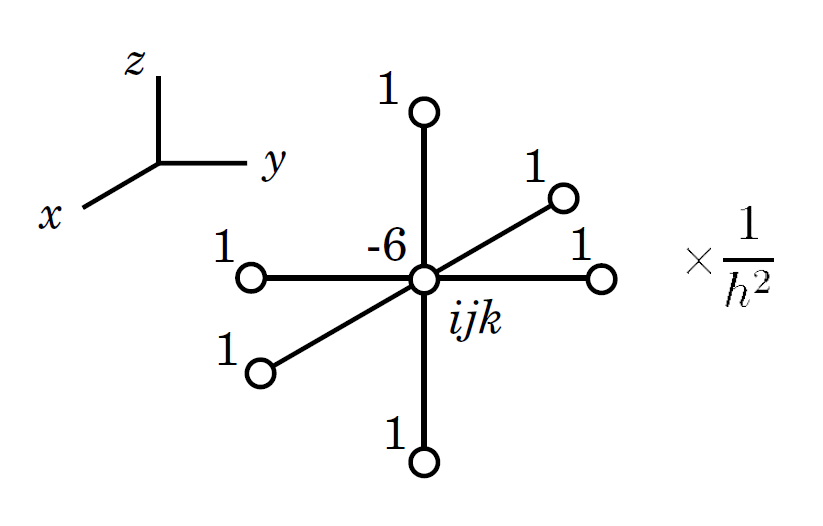
\includegraphics[width=\textwidth]{pictures/3/stencil7}
		\caption{7 points stencil}
		\label{fig:stencil7}
	\end{subfigure}
	\hfill
	\begin{subfigure}[b]{0.45\textwidth}
		\centering
		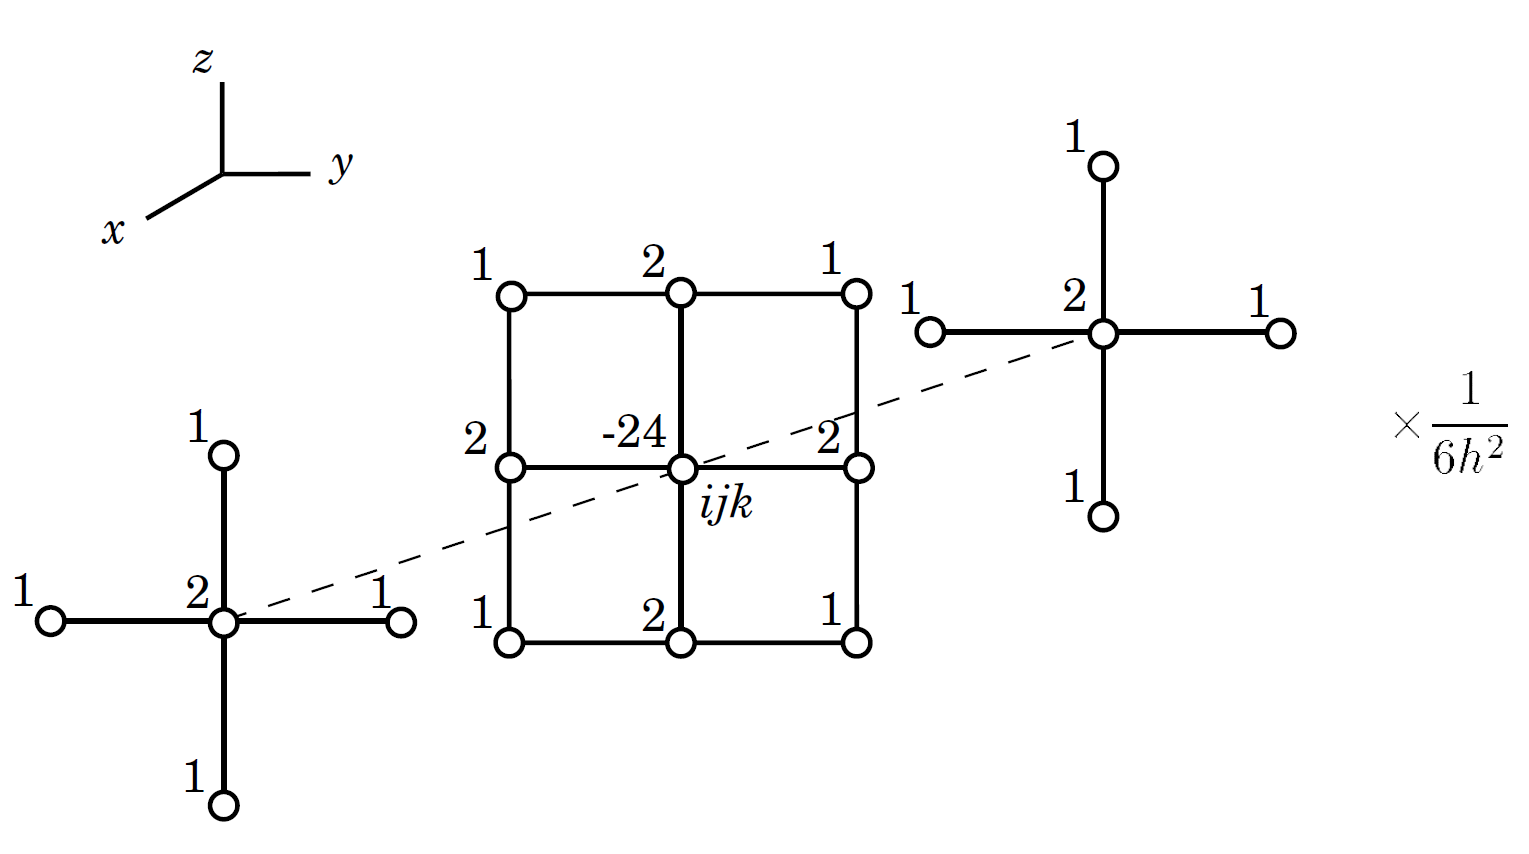
\includegraphics[width=\textwidth]{pictures/3/stencil19}
		\caption{19 points stencil}
		\label{fig:stencil19}
	\end{subfigure}
	\hfill
	\bigskip
	
	\begin{subfigure}[b]{0.45\textwidth}
		\centering
		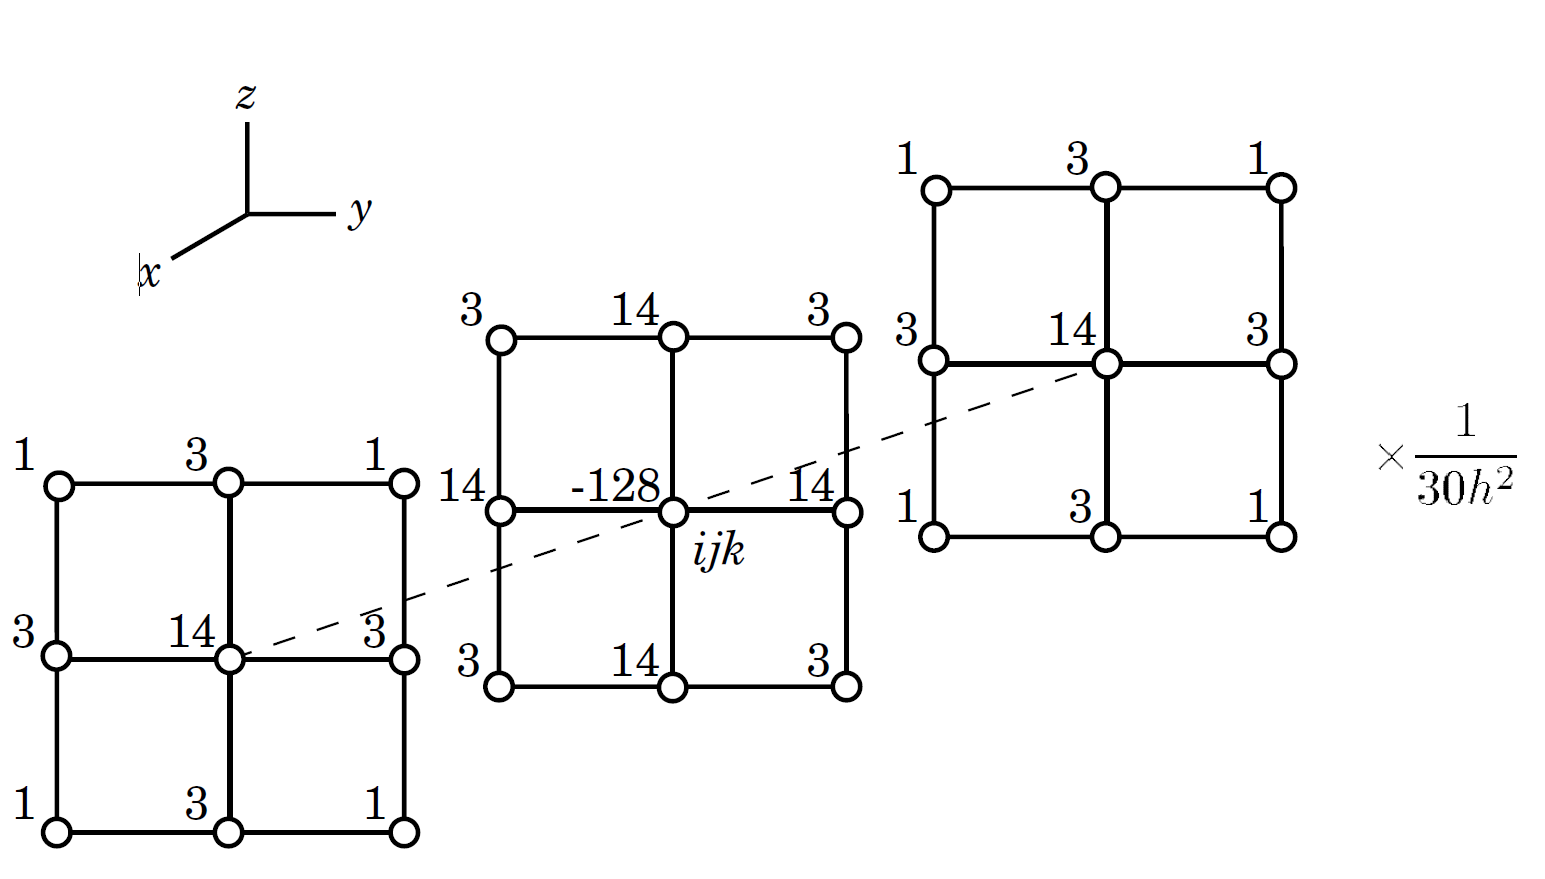
\includegraphics[width=\textwidth]{pictures/3/stencil27}
		\caption{27 points stencil}
		\label{fig:stencil27}
	\end{subfigure}
	\hfill
	
	\caption{CDS and HOC stencils described in Spotz's dissertation.\cite{spotz1996hoc}}
	\label{fig:stencils}
\end{figure}

\subsection{Eigensolvers}
Hereafter, for the sake of simplicity, the sampled wavefunction flattened to a vector of $N \times N \times N$, \textbf{x} is defined to represent $\psi(x,y,z)$. What is left is calculating eigenvalues and eigenvectors using numerical methods. As stated before the time-independent Schr{\"o}dinger equation is:

\begin{equation}
	\hat{H} \psi(x,y,z) = E \psi(x,y,z)
\end{equation}

\noindent which is an eigenproblem, that is the transformation of wavefunction by Hamiltonian results in wavefunction's version multiplied by scalar, which is eigenstate's energy. Because of discretization, the Hamiltonian can be treated as a matrix, and the wavefunction becomes a vector. To solve this for $E$, both sides of the equation are multiplied by $\psi^T(x,y,z).$

\begin{equation}
	\psi^T(x,y,z) \hat{H} \psi(x,y,z) = \psi^T(x,y,z) E \psi(x,y,z)
\end{equation}

\noindent note that $\psi^T(x,y,z)\psi(x,y,z)$ is a scalar, which means that E can be factored out on the right side

\begin{equation}
	\psi^T(x,y,z) \hat{H} \psi(x,y,z) = E(\psi^T(x,y,z) \psi(x,y,z))
\end{equation}

\noindent and both sides divided by also a scalar value of $\psi^T(x,y,z) \psi(x,y,z)$, which is an L2 norm of $\psi(x,y,z)$. After division, the equation becomes:

\begin{equation}
	E = \frac{\psi^T(x,y,z) \hat{H} \psi(x,y,z)}{\psi^T(x,y,z) \psi(x,y,z)}
\end{equation}

\noindent that is a Rayleigh's quotient, which is used in numerical calculations using computers since Vandergraft\cite{vandergraft1971} publication from 1971. Rayleigh's quotient can also be understood as a function that returns an eigenvalue when given an eigenvector.

\begin{equation}
	\lambda_i = R(\textbf{x}_i)
\end{equation}

\noindent

\subsubsection{Gradient descent method}
%TODO citing
Iterative methods were employed to minimize the aforementioned quotient. The most basic algorithm, used for such tasks is gradient descent.\cite{gradient_descent} The algorithm idea is to have an initial guess of what the eigenvector might be. If no such information exists, an uniform random vector should be used. Then, the gradient of Rayleigh's quotient should be calculated. Since the gradient points in the direction where the function grows the fastest, and the algorithm tries to minimize the value, the gradient for the current $\textbf{x}$ iteration is calculated, negated, and multiplied by the learning rate. Thus, the next value of $\textbf{x}^{k+1}$ is:

\begin{equation}
	\textbf{x}^{k+1} = \textbf{x}^{k} - lr \cdot \nabla R(\textbf{x}^{k})
\end{equation}

\noindent after which the check for convergence is made by checking if the L2 norm of the residue vector is greater than the assumed small, positive tolerance. Once the convergence criterion is satisfied or the maximum number of iterations is achieved, the procedure returns the eigenvalue and eigenvector. This algorithm enables the identification of the local minima of multivariate functions.

\subsubsection{Locally Optimal Block Preconditioned Conjugate Gradient}

The Locally Optimal Block Preconditioned Conjugate Gradient (LOBPCG) method is an efficient and versatile algorithm for solving large-scale symmetric eigenvalue problems. It offers competitive computational costs and memory efficiency compared to the Lanczos method, particularly when computing a single extreme eigenpair. The method performs at least as well as gradient descent.\cite{knyazew2001} Its block-based approach facilitates the use of efficient matrix-matrix operations, making it well-suited for high-performance computing. LOBPCG is highly flexible, supporting variable preconditioning, including for non-symmetric or non-positive-definite cases, and allows warm starts by iteratively improving eigenvector approximations from previous iterations. Widely used in applications such as data clustering, image segmentation, and graph-based signal filtering, LOBPCG is easy to implement and has gained popularity in scientific computing. However, challenges such as increased computational costs for very large block sizes due to orthogonalizations and Rayleigh-Ritz computations highlight the importance of careful parameter selection for optimal performance.\cite{knyazew2017}

Attempts were made to adapt the PyTorch implementation\cite{torch_lobpcg} for the thesis due to the computationally attractive "ortho" variant, which employs the LOBPCG method with orthogonal basis selection, described by Stathopoulos et al.\cite{stathopoulous2002}. Unfortunately, these efforts were unsuccessful due to differences between the Laplacian implementation and the input data requirements of the method. Consequently, the method available in the CuPy module was used instead.\cite{cupy_lobpcg}

\subsubsection{Steepest descent with optimal step}
%TODO
This algorithm was implemented to calculate iteratively the excited states of hydrogen.The method was largely inspired by work of Jin et al, who worked on algorithm that escapes saddle points with logarithmic overhead. The Algorithm 2 presented in this article was implemented.\cite{pgd}

To calculate excited states, the goal function is defined as
\begin{equation}
	\rho\left(\mathbf{x}, \bm{\lambda} \right) = \frac{\mathbf{x}^T\mathbf{A}\mathbf{x}}{\mathbf{x}^T\mathbf{x}} + \bm{\lambda}^T \mathbf{Y}^T \mathbf{x}
\end{equation}
\noindent where $\mathbf{Y}\in\mathbb{R}^{d \times k}$ contains orthogonal vectors defining the subspace orthogonal to the sought solution and $\bm{\lambda}\in\mathbb{R}^k$ is the vector of Lagrange multipliers.
Thus, the gradients read
\begin{equation}
	\nabla_{\mathbf{x}}\rho\left(\mathbf{x},\bm{\lambda}\right) = \frac{2}{\mathbf{x}^T\mathbf{x}}\left(\mathbf{A}-\frac{\mathbf{x}^T\mathbf{A}\mathbf{x}}{\mathbf{x}^T\mathbf{x}}\right)\mathbf{x} + \mathbf{Y}\bm{\lambda},
\end{equation}
\begin{equation}
	\nabla_{\bm{\lambda}}\rho\left(\mathbf{x},\bm{\lambda}\right) = \mathbf{Y}^T\mathbf{x}.
\end{equation}
The search direction for gradient descent is
\begin{equation}
	\mathbf{p}=-\left[\left(\nabla_{\mathbf{x}}\rho\left(\mathbf{x},\bm{\lambda}\right)\right)^T, \left(\nabla_{\bm{\lambda}}\rho\left(\mathbf{x},\bm{\lambda}\right)\right)^T\right]^T = \left[\mathbf{p}_{\mathbf{x}}^T,\mathbf{p}_{\bm{\lambda}}^T\right]^T.
\end{equation}
\noindent The goal as a function of the step size $\delta$ reads
\begin{equation}
	\rho\left(\mathbf{x}+\delta \mathbf{p}_{\mathbf{x}},\bm{\lambda}+\delta \mathbf{p}_{\bm{\lambda}}\right) = \frac{a_1+b_1\delta+c_1\delta^2}{a_2+b_2\delta+c_2\delta^2} + a_3+b_3\delta + c_3 \delta^2,
	\label{eq5}
\end{equation}
where
\begin{align*}
	a_1 &= \mathbf{x}^T\mathbf{A}\mathbf{x}, & \quad a_2 &= \mathbf{x}^T\mathbf{x}, & \quad a_3 &= \bm{\lambda}^T\mathbf{Y}^T\mathbf{x}, \\
	b_1 &= 2 \mathbf{p}_{\mathbf{x}}^T\mathbf{A}\mathbf{x}, & \quad b_2 &= 2\mathbf{p}_{\mathbf{x}}^T\mathbf{x}, & \quad b_3 &=  \mathbf{p}_{\bm{\lambda}} \mathbf{Y}^T \mathbf{x} + \bm{\lambda}\mathbf{Y}^T\mathbf{p}_{\mathbf{x}}, \\
	c_1 &= \mathbf{p}_{\mathbf{x}}^T \mathbf{A} \mathbf{p}_{\mathbf{x}}, & \quad c_2 &= \mathbf{p}_{\mathbf{x}}^T\mathbf{p}_{\mathbf{x}}, &  \quad c_3 &= \mathbf{p}_{\bm{\lambda}}^T\mathbf{Y}^T\mathbf{p}_{\mathbf{x}}.
\end{align*}
Minimization of \ref{eq5} w.r.t. $\delta$ leads to the $5$th order polynomial equation
\begin{equation}
	q_0 + q_1 \delta + q_2 \delta^2 + q_3 \delta^3 + q_4 \delta^4 +q_5 \delta^5 = 0,
\end{equation}
where the coefficients are:
\begin{align*}
	q_0 &= -a_1 b_2 + a_2 (b_1 + a_2 b_3),\\
	q_1 &= -2 a_1 c_2 + 2 a_2 (b_2 b_3 + c_1 + a_2 c_3),\\ 
	q_2 &= b_2^2 b_3 + b_2 c_1 - b_1 c_2 + 2 a_2 b_3 c_2 + 4 a_2 b_2 c_3, \\
	q_3 &= 2 (b_2 b_3 c_2 + b_2^2 c_3 + 2 a_2 c_2 c_3),\\
	q_4 &= c_2 (b_3 c_2 + 4 b_2 c_3),\\
	q_5 &= 2 c_2^2 c_3.
\end{align*}
\noindent which facilitates the calculation of the optimal step size.

% ale ja liczę w całości gradienty, to jaki ma związek stochastyczny gradient
\subsubsection{Stochastic gradient descent}

Although not implemented in this work, stochastic gradient descent description is crucial for understanding the following minimizing algorithm, that is Adam. The idea comes from Robbins-Monroe\cite{robbins-monroe} algorithm of stochastic approximation. It's useful when dealing with high-dimensional problems, reducing the 

\subsubsection{Adam}

Adam algorithm is a refinement of stochastic gradient descent (SGD) algorithm. The idea of
Adam, derived from adaptive moment estimation, is a refinement of basic gradient descent algorithm. It characterizes itself by the adaptive learning rates using first and second moments of gradients, while still requiring only first-order gradients. It's also has low memory requirements. It combines two gradient descent methodologies, that is momentum and Root Mean Square Propagation (RMSP).



\begin{align*}
		&m_w^{(t+1)} = \beta_1 m_w^{(t)} + (1 - \beta_1) \nabla_w L^{(t)} \\
		&v_w^{(t+1)} = \beta_2 v_w^{(t)} + (1 - \beta_2) (\nabla_w L^{(t)})^2 \\
		&\hat{m_w} = \frac{m_w^{(t+1)}}{1-\beta_1^t} \\
		&\hat{v_w} = \frac{v_w^{(t+1)}}{1-\beta_2^t} \\
		&w^{(t+1)} = w^{(t)} - \eta \frac{\hat{m_w}}{\sqrt{\hat{v_w}} + \epsilon}
\end{align*}

\cite{kingma_adam:_2017}
\cite{adam_geeks}

\subsection{Tools and techniques}

\subsubsection{Python}

The primary programming language used in this work was Python. This programming language is widely recognized as a programming language used by scientists and engineers. Moreover, the abundance of Python modules, such as NumPy, SciPy, MatPlotLib, etc., makes it an incredibly versatile language. Its high readability, simple syntax, and gentle learning curve allow STEM-related field practitioners to enter programming without delay.

Python is a convenient tool for integrating many scientific and technical computing functionalities. The modules used, Mayavi and MatPlotLib for visualization, NumPy and CuPy for numerical computations, and direct access to CUDA via CuPy might not be available in other programming languages. Moreover, the vibrant community provides a steady flow of fixes and improvements, reference documentation, and many forums with resources and support that foster collaboration among researchers and developers.\cite{python}

\subsubsection{CuPy}

CuPy provides the functionality of NumPy and SciPy modules, offering GPU-accelerated computing with Python. It works on both Nvidia CUDA and AMD ROCm platforms. Its API is compatible with the aforementioned modules.\cite{cupy_overview} CuPy also provides an easy way of implementing custom kernel functions. For example, in "Learn CUDA" book by Han et al., the ElemenwiseKernel, the simplest way of implementing CUDA kernel is described:\cite{learn_cuda}

\vspace{0.2cm}
\lstinputlisting[caption=Simple element-wise kernel, label=listing1, captionpos=b]{listings/3/listing1.py}
which takes two arguments, x and y, calculates it's squared difference. It is worth noting, values are not returned directly, instead a reference to a location where the result will be stored has to be provided, in this example, in variable z.

Also it is possible to use raw kernel functions. Raw kernels are used when one wants to define a custom kernel that executes CUDA source code. Using raw kernels allows for control of grid size, block size, shared memory size, and stream. An example of the raw kernel from CuPy docs\cite{cupy_raw_kernel}:

\vspace{0.2cm}
\lstinputlisting[caption=Example code of raw kernel that performs addition of two 2D arrays., label=listing2, captionpos=b]{listings/3/listing2.py}

Moreover, CuPy provided the TextureObject\cite{cupy_texture} and SurfaceObject\cite{cupy_surface}, allowing the CUDA textures and surfaces to be passed into the raw kernel. The relevance of this will be addressed in more depth in the next section. Also, the LOBPCG implementation from this module was used.\cite{cupy_lobpcg}


\subsubsection{CUDA}

In this work, we meet the case of data parallelism\cite{cheng2014professional}, which is a situation where calculation time might benefit when many data items are operated at the same time. The CUDA approach for such problems is to provide each thread with equal parts of data so that every thread can work on its part simultaneously.

An important issue with parallel computation has been raised by members of high performance computing (HPC) community. Kogge et al. noted that rise of the \textit{flop to byte ratio} (F2B), defined as floating-point operations per second (FLOPS) divided by the available memory bandwith (in bytes per second) in hardware is a recognized challenge in high performance computing. Moreover, the development of dynamic random-access memory (DRAM) in recent years was a tradeoff of higher bandwith for lower latency.\cite{kogge2008exascale} It is especially important in algorithms that characterize in high memory utilization compared to the number of arithmetic instructions done and puts pressure on scientists to design algorithms efficient not only from computational, but also space complexity.\cite{krotkiewski2011efficient}

\vspace{0.2cm}

\begin{table}[!ht]
	\centering
	\caption{Comparison of FLOP, Memory Bandwidth, and FLOP-to-Byte Ratio for NVIDIA GPUs}
	\label{tab:gpu-comparison}
	\resizebox{\textwidth}{!}{%
		\begin{tabular}{|l|c|c|c|}
			\hline
			\textbf{GPU Model}         & \textbf{FLOP (TFLOPS)} & \textbf{Memory Bandwidth (GB/s)} & \textbf{FLOP-to-Byte Ratio (FLOP/byte)} \\ \hline
			NVIDIA Tesla C2050         & 1.03                   & 144                              & 7.15                                    \\ \hline
			NVIDIA RTX A4000           & 19.2                   & 448                              & 42.9                                    \\ \hline
			NVIDIA TITAN RTX           & 16.3                   & 672                              & 24.2                                    \\ \hline
			NVIDIA GeForce RTX 4090    & 82.6                   & 1,010                            & 81.8                                    \\ \hline
			
		\end{tabular}%
	}
	\smallskip
	\small \textit{Source}: Own elaboration based on techpowerup.com publications\cite{techpowerup1}\cite{techpowerup2}\cite{techpowerup3}
\end{table}

Since the publication of Krotkiewki's findings, the problem only was exacerbated. The NVIDIA Tesla C2050 mentioned in his article has half of F2P compared to it's current successor, NVIDIA RTX A4000. Moreover, the GPUs utilized in this work were characterized by even higher F2P, further highlighting the growing disparity between computational power and memory bandwidth.

% TODO mogę tutaj opisać CUDA memory model, texturę i surface, jeżeli za mało treści

Using aforementioned HOC stencils from Spotz dissertation\cite{spotz1996hoc}, there is high probability that produced code will be cache-friendly, since the memory reads are characterized by high locality, that is the adjacent values stored in memory are read. Still, in the case of cache miss, the algorithms implemented had to provide as low memory latency as possible. For that purpose, the findings of Akhtar et al. were employed. In his work on "Efficient Memory Access Patterns for Solving 3D Laplace Equation on GPU", he implemented 12 kernels with different with unique memory access pattern. In his publication, the best performing kernel achieved a speedup of 70 times with comparison to CPU code\cite{akhtar2018efficient}. The listing of this kernel is as follows:

\vspace{0.2cm}
\lstinputlisting[caption=Listing of kernel K5 for solving Laplace 3D.\cite{akhtar2018efficient}, label=listing3, captionpos=b]{listings/3/listing3.py}

Achieved results were attributed to efficient use of available memory spaces in GPU, best cache hit rate, which facilitated highest GPU throughput. The CuPy kernel function for Laplace operator in this work was done based on presented Akhtar's findings.